%%%%%%%%%%%%%%%%%%%%%%%%%%%%%%%%%%%%%%%%%%%%%%%%%%%
%% P3: Phenomenology of Particle Physics                         
%%
%% Author:  André Rubbia                   		 
%%
%% Figure 19.23 Graphical representation of the relationship between parton $(x,Q^2)$ variables and the 
%% kinematical variables corresponding to a final state of invariant mass $M$ produced with rapidity $y$ 
%% at the LHC collider with $\sqrt{s} = 13$~TeV
%%
%% This work is licensed under the Creative Commons Attribution 4.0 International License. 
%% To view a copy of this license, visit http://creativecommons.org/licenses/by/4.0/ or 
%% send a letter to Creative Commons, PO Box 1866, Mountain View, CA 94042, USA.
%%
%%%%%%%%%%%%%%%%%%%%%%%%%%%%%%%%%%%%%%%%%%%%%%%%%%%

\documentclass[a4paper,10pt]{article}

\usepackage[T1]{fontenc}
\usepackage[utf8]{inputenc}
\usepackage{lmodern}
\usepackage[labelfont=bf]{caption}
\usepackage{upgreek}

\usepackage{tikz}
\usepackage{pgfplots}
\pgfplotsset{compat=1.17}
\usepgfplotslibrary{ternary}
\usepgfplotslibrary{fillbetween}
\usepgfplotslibrary{external}

\def\d{\mathrm{d}}

\begin{document}

%%%%%%%%%%%%%%%%   FIGURE  %%%%%%%%%%%%%%%%%%%%%%%%%%%%%%
\begin{figure}[htb]
\centering
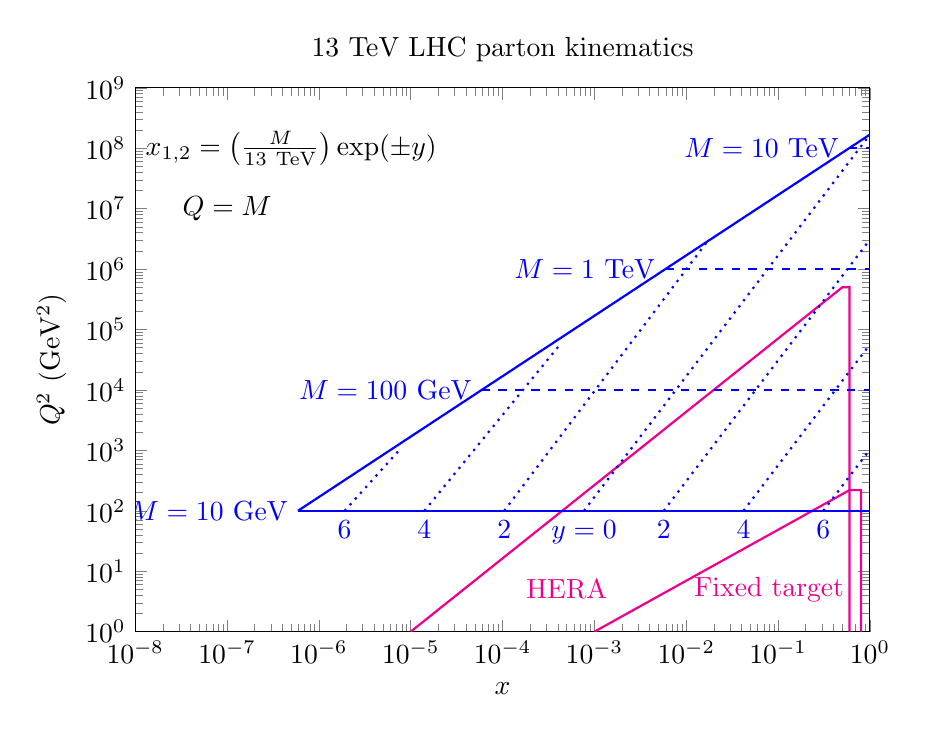
\begin{tikzpicture}[scale=1.]
\begin{loglogaxis}[
        width=0.9\textwidth,
        height=0.7\textwidth,
	title=13 TeV LHC parton kinematics,
	ytick={1e0, 1e1, 1e2, 1e3,1e4,1e5,1e6,1e7,1e8,1e9},
	ymin=1e0, ymax=1e9,
	xmin=1e-8, xmax=1,
	xlabel=$x$,
	ylabel={$Q^2$  (GeV$^2$)}
	]
	\draw[thick,magenta] (axis cs:1e-3,1e0) -- (axis cs:0.6,220) -- (axis cs:0.8,220) -- (axis cs:0.8,1);
	\draw[thick,magenta] (axis cs:1e-5,1e0) -- (axis cs:0.5,5e5) -- (axis cs:0.6,5e5) -- (axis cs:0.6,1);
	\draw[thick,blue] (axis cs:10/13000*10/13000,1e2) node[left] {$M=10$~GeV} -- (axis cs:1,1e2);
	\draw[thick,blue] (axis cs:10/13000*10/13000,1e2) -- (axis cs:1,1.69e8);
	\draw[thick,blue,dashed] (axis cs:100/13000*100/13000,1e4) node[left] {$M=100$~GeV~}  -- (axis cs:1,1e4);
	\draw[thick,blue,dashed] (axis cs:1000/13000*1000/13000,1e6) node[left] {$M=1$~TeV~}  -- (axis cs:1,1e6);
	\draw[thick,blue,dashed] (axis cs:10000/13000*10000/13000,1e8)node[left] {$M=10$~TeV~}   -- (axis cs:1,1e8);
% y=0
	\draw[thick,blue,dotted] (axis cs:10/13000,1e2) node[below] {$y=0$} -- (axis cs:1,1.69e8);
% y=2 exp(2)=7.389
	\draw[thick,blue,dotted] (axis cs:10/13000*7.389,1e2) node[below] {$2$} -- (axis cs:1,1.69e8/7.389/7.389);
% y=4, exp(4)=54.598150
	\draw[thick,blue,dotted] (axis cs:10/13000*54.598150,1e2) node[below] {$4$}  -- (axis cs:1,1.69e8/54.598150/54.598150);
% y=6, exp(6)=403.428793
	\draw[thick,blue,dotted] (axis cs:10/13000*403.428793,1e2) node[below] {$6$}  -- (axis cs:1,1.69e8/403.428793/403.428793);
% y=-2 exp(2)=7.389
	\draw[thick,blue,dotted] (axis cs:10/13000/7.389,1e2) node[below] {$2$}  -- (axis cs:1.69e3/13000/7.389,1.69e8/7.389/7.389);
% y=-4, exp(4)=54.598150
	\draw[thick,blue,dotted] (axis cs:10/13000/54.598150,1e2) node[below] {$4$}  -- (axis cs:3.e2/13000/54.598150,1.69e8/54.598150/54.598150);
% y=-6, exp(6)=403.428793
	\draw[thick,blue,dotted] (axis cs:10/13000/403.428793,1e2) node[below] {$6$} -- (axis cs:40/13000/403.428793,1.69e8/403.428793/403.428793);
	\node[magenta] at (axis cs:5e-4,5) {HERA};
	\node[magenta] at (axis cs:8e-2,5) {Fixed target};
	\node at (axis cs:5e-7, 1e8) {$x_{1,2}=\left(\frac{M}{13~\mathrm{TeV}}\right)\exp(\pm y)$};
	\node at (axis cs:1e-7, 1e7) {$Q=M$};
\end{loglogaxis}
\end{tikzpicture}
\caption{Graphical representation of the relationship between parton $(x,Q^2)$ variables and the kinematical variables corresponding to a final state of invariant mass $M$ produced with rapidity $y$ at the LHC collider with $\sqrt{s} = 13$~TeV.}
\end{figure}
%
%%%%%%%%%%%%%%%%   END FIGURE  %%%%%%%%%%%%%%%%%%%%%%%%%%%%%%
%
\end{document}
